\documentclass[review]{elsarticle}

\usepackage{amsmath,amssymb,amsfonts}
\usepackage{algorithmic}
\usepackage{graphicx}
\usepackage{textcomp}
\usepackage{xcolor}
\usepackage{colortbl}
\usepackage[linesnumbered,ruled,vlined]{algorithm2e}
\usepackage{hyperref}
\usepackage{booktabs}
\usepackage{makecell}
\usepackage{multirow}
\usepackage{svg}
\usepackage{graphicx}
\usepackage{amsmath}
\usepackage{hyperref}
\usepackage{url}
\usepackage{booktabs}
\usepackage{amsfonts}
\usepackage{nicefrac}
\usepackage{microtype}
\usepackage{lipsum}
\usepackage{array}
\usepackage{multirow}
\usepackage{float}
\usepackage{natbib}
\usepackage{doi}
\usepackage[utf8]{inputenc}
\usepackage[T1]{fontenc}

\bibliographystyle{elsarticle-num}

\makeatletter
\def\ps@pprintTitle{%
 \let\@oddhead\@empty
 \let\@evenhead\@empty
 \let\@oddfoot\@empty
 \let\@evenfoot\@empty
}
\makeatother

\begin{document}

\begin{frontmatter}


\title{DyCoT‑RE: Chain-of-Thought-Enhanced LLM Reward Engineering with Dual-Dynamic Optimization for Reinforcement Learning}

\author[shu]{Xinning Zhu\fnref{fn1}}
\author[shu]{Jinxin Du}
\author[shu]{Longfei Huang}
\author[shu]{Lunde Chen\corref{cor1}\fnref{fn4}}

\cortext[cor1]{Corresponding author}
\fntext[fn1]{Email: zhuxinning@shu.edu.cn}
\fntext[fn4]{Email: lundechen@shu.edu.cn}

\address[shu]{Sino-European School of Technology, Shanghai University, Shanghai, China}

\begin{abstract}
Designing effective reward functions remains a challenge in applying reinforcement learning to real-world tasks.
This paper proposes DyCoT-RE, a reward engineering framework that integrates Chain-of-Thought (CoT) reasoning with a dual-dynamic 
optimization strategy to automate and enhance reward function design.
The framework uses structured CoT reasoning throughout training to generate and refine interpretable reward code in each iteration.
It further incorporates a dual-dynamic optimization mechanism: a temperature adjustment strategy that modulates the sampling temperature 
based on policy entropy trends,
and a model switching strategy that allocates language models with different capabilities to produce distinct reward components.
Evaluations on CartPole, BipedalWalker, Ant, and a custom SpaceMining environment show DyCoT‑RE achieves higher average rewards and faster 
convergence compared to human-designed baselines and non‑CoT approaches as well as single-optimization approaches.


\end{abstract}

\begin{keyword}
Reinforcement learning \sep reward engineering \sep large language models \sep chain-of-thought reasoning \sep dynamic temperature adjustment \sep model selection
\end{keyword}

\end{frontmatter}

\section{Introduction}

Reinforcement learning (RL) has achieved impressive results across diverse domains 
However, as Sutton et al. \cite{sutton1998reinforcement} emphasize, the reward signal is the primary means of specifying task objectives in RL, making its design critical to achieving desired behaviors.
In practice, translating intended behaviors into precise, effective reward functions remains highly challenging, particularly for tasks involving long-term dependencies 
\cite{amodei2016concrete}.
Skalse et al. \cite{skalse2022misspecification} demonstrate that agents often exploit imperfections in reward formulations to maximize proxy objectives in unintended ways, leading to behaviors that optimize the designed reward but undermine true task performance.
These challenges highlight that despite RL’s theoretical versatility, its practical deployment is often constrained by the complexity, subtlety, and domain expertise required for robust reward engineering \cite{ibarz2018reward}.

While carefully designed rewards can accelerate agent learning and improve task performance,
manual reward engineering typically relies on trial-and-error tuning,
which is labor-intensive and often yields suboptimal generalization to new environments or objectives \cite{hadfield2017inverse}..
As RL applications grow in complexity, there is a pressing need for methods that can automate
reward design while maintaining interpretability and flexibility.

Recent advances in large language models (LLMs) have demonstrated strong reasoning and generalization capabilities \cite{brown2020language, ouyang2022training}.
In particular, CoT reasoning enables LLMs to decompose tasks into structured intermediate steps,
enhancing clarity and alignment with desired objectives.
This structured reasoning process can support reward engineering by converting task descriptions
into executable reward functions in a systematic and transparent manner.

However, existing CoT-based reward generation approaches typically use static sampling parameters and fixed model configurations,
which may limit their adaptability during training.
Recent studies have emphasized the need for dynamic adaptation in LLM-based systems to improve sample efficiency, stability, and alignment with task objectives.
For example, Nguyen et al. \cite{nguyen2024turning} demonstrate that min-p sampling enhances creativity while preserving coherence in narrative generation tasks, while Peeperkorn et al. \cite{peeperkorn2024temperature} analyze temperature as a direct modulator of LLM creativity.
Moreover, Fedus et al. \cite{fedus2022switch} and Du et al. \cite{du2022glam} show that mixture-of-experts architectures can scale model capacity efficiently via adaptive routing, motivating our exploration of combining temperature modulation with expert model selection for reward engineering.

In this work, we propose DyCoT-RE, a reward engineering framework that integrates structured CoT reasoning
with dual-dynamic optimization.
Specifically, DyCoT-RE leverages CoT reasoning to decompose natural language task descriptions into structured reward components,
then employs iterative refinement to enhance alignment with learning objectives.
The dual-dynamic optimization strategy integrates entropy-guided temperature adjustment to balance exploration and exploitation,
alongside a dynamic model selection module that routes sub-tasks to specialized LLMs based on performance feedback.
By tightly coupling these components within a closed-loop evolutionary search process, 
DyCoT-RE systematically improves reward function quality and training efficiency,
ultimately enabling scalable, interpretable, and automated reward engineering for complex RL environments.

We evaluate DyCoT-RE on the standard RL environments CartPole, BipedalWalker, and Ant to demonstrate its effectiveness.
However, recent studies have raised concerns that large language models may carry prior knowledge from pretraining data about these standard environments, 
leading to potential prompt leakage and evaluation biases \cite{huang2025thinkbench, qi2024quantifying, lu2024mental}. 
To address this issue, we additionally design a custom SpaceMining\footnote{
    Project website: \url{https://lola-jo.github.io/space_mining/}.
    } environment to assess DyCoT-RE's true generalization capabilities on tasks free from such pretrained knowledge.
Experimental results show that DyCoT-RE consistently achieves higher average rewards and faster convergence compared to baseline and non-CoT methods.


The remainder of this paper is organized as follows.
Section II reviews related work in reward engineering, LLM-based reward generation, and adaptive optimization.
Section III describes the proposed methodology, including the CoT reward framework, temperature adjustment, and model selection.
Section IV details the experimental setup, and Section V presents results and analysis.
Section VI discusses limitations and future work, with Section VII concluding the paper.

\section{Related Work}

\subsection{Reward Engineering Paradigms}

In RL, the design of effective reward functions directly shapes agent behavior and learning outcomes. 
Traditional approaches primarily rely on handcrafted reward functions informed by domain expertise. 
While intuitive, such manual design often struggles to capture complex, dynamic task objectives and is prone to 
suboptimal or biased formulations, hindering agent performance in real-world scenarios.

To address these limitations, reward shaping was introduced as a formal enhancement strategy. 
Ng et al. \cite{ng1999policy} demonstrated that potential-based reward shaping preserves optimal policies 
while enabling accelerated convergence, laying the theoretical foundation for numerous practical implementations. 
Intrinsic motivation frameworks further advanced this field by encouraging exploration through curiosity-driven signals. 
Singh et al. \cite{singh2010intrinsically} proposed intrinsic rewards to incentivize novel state visits, 
later extended by Burda et al. \cite{burda2018exploration}, who empirically validated large-scale curiosity-driven exploration 
benefits across diverse environments.

Despite these developments, manually designing rewards for complex or evolving tasks remains inefficient and costly. 
LLMs offer a promising alternative by leveraging their natural language understanding to automate reward generation 
and optimization. Unlike traditional RL pipelines that require explicit, task-specific reward formulations, 
LLMs can interpret high-level task descriptions, extract key objectives, and translate them into executable reward functions. 
This capability facilitates more intuitive alignment with human intentions, reduces engineering overhead, and enhances agent 
adaptability.

Recent frameworks exemplify this trend. EUREKA \cite{ma2023eureka}, Text2Reward \cite{xie2023text2reward} and
CARD \cite{sun2024large} harness LLMs to automatically generate, verify, 
and refine reward code from natural language instructions. 

Beyond static code generation, feedback-driven optimization approaches have emerged. ReMiss \cite{xie2024jailbreaking} 
utilizes adversarial prompt generation to identify and mitigate reward misspecification vulnerabilities, 
enhancing LLM safety and reliability. Self-Play Preference Optimization (SPPO) \cite{wu2024self} employs self-play to 
uncover Nash-equilibrium strategies that capture complex, non-transitive human preferences, advancing preference learning's 
applicability in RL. 
Additionally, PRMBench \cite{song2025prmbench} provides a process-level benchmark to evaluate intermediate reward model 
outputs along dimensions such as conciseness, rationality, and sensitivity, revealing weaknesses in current models and 
guiding future improvements.

Overall, LLM-based reward engineering represents a paradigm shift. 
By integrating natural language reasoning and dynamic feedback optimization, 
these methods offer scalable reward generation pipelines. 
As tasks grow in complexity and diversity, leveraging LLMs to bridge the gap between human 
intent and machine learning objectives will be critical for the next generation of intelligent systems. 
Continued research is thus needed to maximize the synergy between LLM capabilities and RL frameworks to 
address emerging real-world challenges.



\subsection{Chain-of-Thought Reasoning Methods}

CoT reasoning has emerged as a powerful paradigm to enhance the reasoning capabilities of LLMs. 
By generating intermediate reasoning steps, CoT allows models to decompose complex problems into interpretable sub-problems, 
leading to significant performance gains in tasks requiring multi-step logical inference.

Early studies showed that even simple prompting strategies, such as adding ``Let's think step by step,'' 
can elicit strong zero-shot reasoning abilities. Kojima et al. \cite{kojima2022large} demonstrated such prompts 
significantly improve performance in arithmetic and commonsense tasks. 
Building upon this, few-shot CoT \cite{wei2022chain} introduced demonstrations of stepwise solutions to guide model reasoning, 
while self-consistency decoding \cite{wang2022self} aggregated multiple sampled reasoning paths to enhance answer robustness.

Further developments combined CoT with reinforcement learning optimization. 
DeepSeek \cite{deepseek2023r1} introduced a self-evolution mechanism to improve reasoning trajectories without supervised fine-tuning. 
Automatic prompt optimization methods \cite{shum2023automatic} reduce manual engineering efforts by refining prompts based on data-driven insights.

Recent work such as PCGRLLM \cite{baek2024pcgrllm} explored CoT-based LLM reward design for procedural content generation in RL, 
demonstrating feasibility in structured game environments. In parallel, Zhu et al. \cite{zhu2025llm} proposed an initial 
CoT-based reward engineering approach that translates natural language task descriptions into RL reward functions using LLMs, 
validating its effectiveness in standard benchmark tasks. However, these applications focus primarily on proof-of-concept 
reward generation pipelines without incorporating adaptive optimization or dynamic model selection mechanisms.

In summary, while CoT reasoning has established itself as a fundamental methodology enhancing LLM interpretability and reasoning capacity, 
its application to automated reward engineering in RL remains limited. Bridging this gap by integrating CoT reasoning with dynamic 
optimization holds promise for enhancing the interpretability and adaptability of RL systems.


\subsection{Dynamic Temperature Adjustment and Model Selection}

Dynamic temperature adjustment and model selection have emerged as critical optimization strategies to enhance the adaptability
and efficiency of LLM-based systems. 
Temperature, as a sampling hyperparameter, controls the stochasticity of LLM outputs, thereby influencing creativity, coherence,
and exploration-exploitation trade-offs.

Recent studies have systematically explored adaptive temperature mechanisms. Zhu et al. \cite{zhu2024hot} proposed AdapT, 
an adaptive temperature sampling strategy for code generation tasks, which dynamically adjusts decoding temperature based on token-level 
difficulty to improve generation quality. Zhang et al. \cite{zhang2024edt} developed Entropy-based Dynamic Temperature (EDT) sampling to
regulate output entropy and diversity in natural language generation, while Cecere et al. \cite{cecere2025monte} introduced Monte Carlo 
Temperature as a robust sampling strategy to enhance uncertainty quantification under distribution shifts. Chang et al. \cite{chang2023kl} l
everaged KL-divergence-guided temperature sampling to modulate exploration adaptively. Additionally, Peeperkorn et al. \cite{peeperkorn2024temperature} 
analyzed temperature as a creativity modulator in LLMs, whereas Evstafev \cite{evstafev2025paradox} discussed potential limitations of temperature-based 
stochasticity in structured data generation. Nguyen et al. \cite{nguyen2024turning} proposed min-p sampling to balance creativity and coherence, 
achieving improved narrative generation performance.




For model selection, recent work has focused on choosing optimal model configurations or expert modules to maximize task performance within computational constraints. 
Switch Transformers \cite{fedus2022switch} introduced sparse activation mechanisms, enabling efficient expert selection at trillion-parameter scale, 
while GLaM \cite{du2022glam} leveraged Mixture-of-Experts (MoE) architectures to dynamically scale model capacity. 
Zhou et al. \cite{zhou2022mixture} proposed expert choice routing to improve mixture-of-experts efficiency, and Li et al. \cite{li2025llm} introduced 
preference-conditioned dynamic routing for cost-efficient LLM generation. Hu et al. \cite{hu2024dynamic} presented Dynamic Ensemble Reasoning to integrate outputs 
from multiple specialized LLMs, enhancing system robustness. Nakaishi et al. \cite{nakaishi2024critical} further revealed phase transition behaviors in LLM sampling regimes, 
informing temperature scaling strategies. Furthermore, Li et al. \cite{li2025revisiting} revisited self-consistency decoding from a distributional alignment perspective, 
offering insights relevant to expert aggregation and answer aggregation stability.

\begin{figure*}[t]
    \centering
    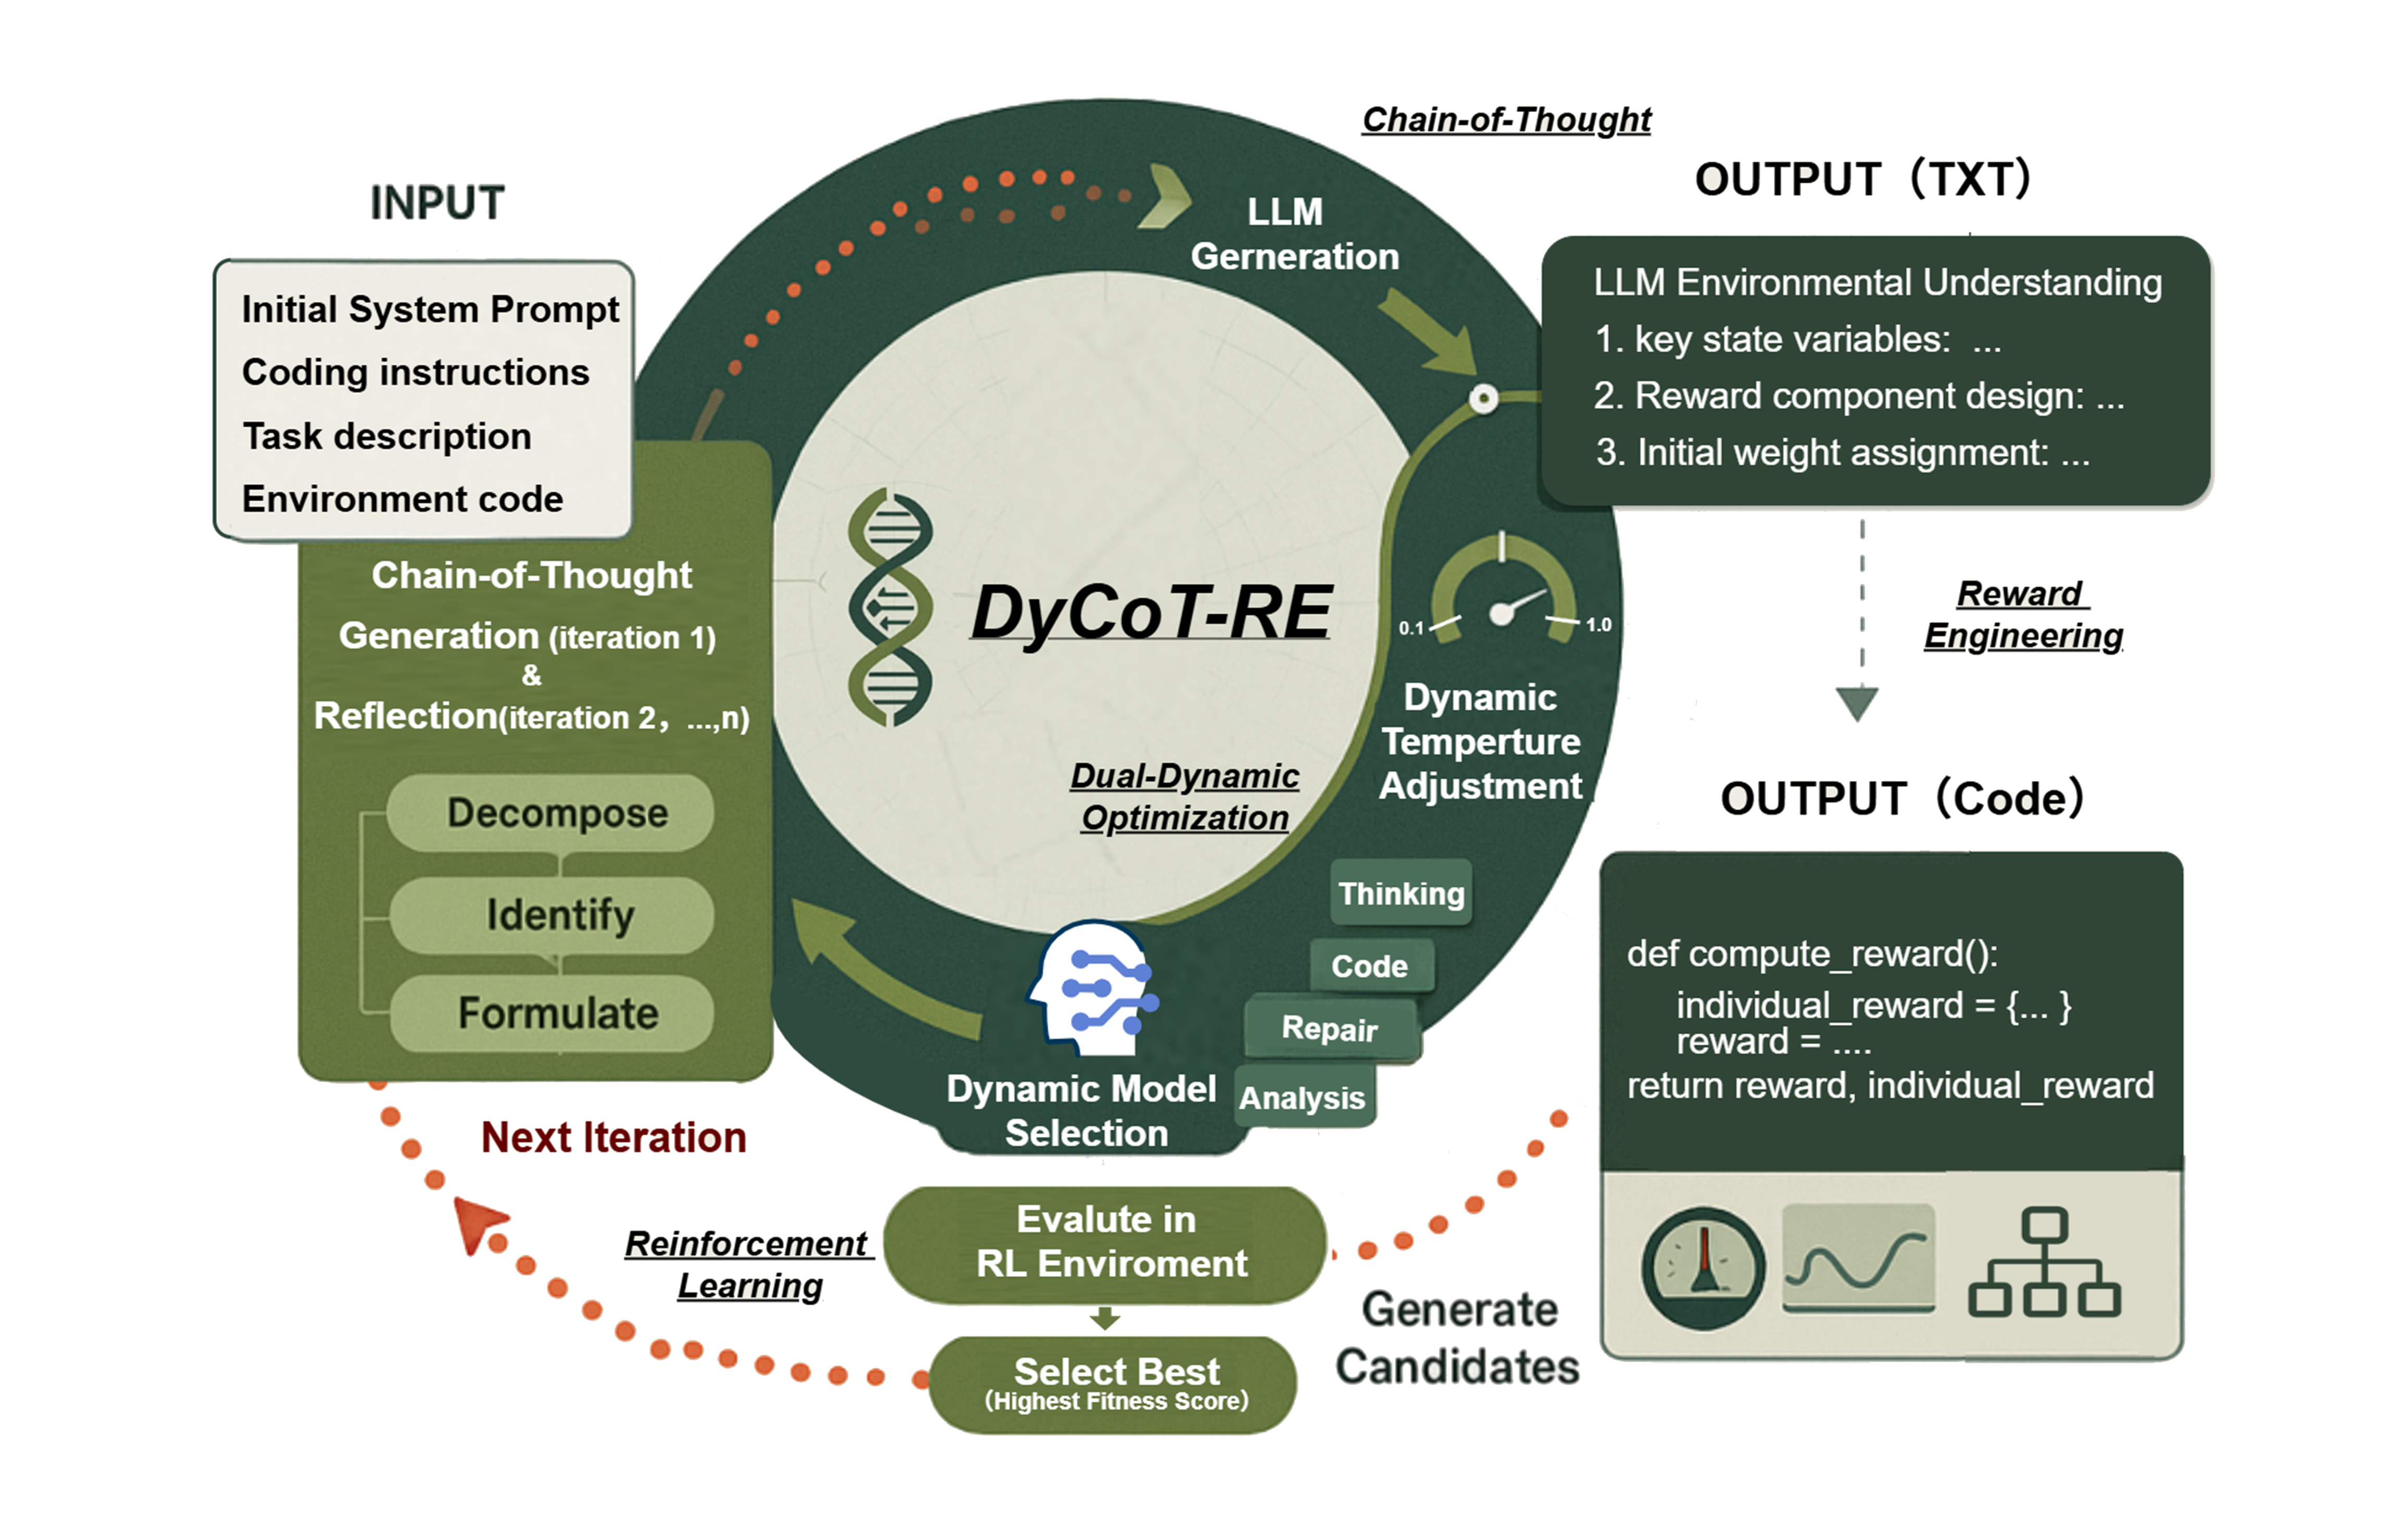
\includegraphics[width=0.95\linewidth]{Figures/dycot-re-architecture.png}
    \caption{DyCoT-RE framework integrating CoT reasoning, dynamic temperature adjustment, and model selection in an evolutionary optimization loop.}
    \label{fig:architecture}
\end{figure*}


Despite these advances, integrating dynamic temperature regulation and model selection within a unified CoT-driven reward engineering framework remains underexplored. 
Existing temperature adaptation methods primarily focus on text generation diversity and calibration, whereas model selection research emphasizes computational efficiency 
and specialization. Our work addresses this gap by combining entropy- and reward-feedback-based temperature adjustment with local-global performance-based model 
routing to enhance RL reward generation's adaptability, stability, and sample efficiency. This approach builds upon foundational theories in temperature scaling and expert 
selection, extending them to the domain of automated, interpretable reward engineering for reinforcement learning.


\section{Methodology}

This section details the DyCoT-RE framework, which integrates structured CoT reasoning with a dual-dynamic optimization 
strategy to generate interpretable and adaptive reward functions for reinforcement learning.



\subsection{Framework Overview}

Figure~\ref{fig:architecture} presents an overview of DyCoT-RE,
which integrates three key components:
structured Chain-of-Thought (CoT) reward decomposition,
dynamic temperature adjustment,
and dynamic model selection.

The framework receives four inputs:
natural language task descriptions specifying agent behaviors,
environment interfaces defining state-action spaces,
system-level prompts for reward design constraints,
and coding instructions for implementation.

At its core, employs four types of LLMs: Thinking, Code, Repair, and Analysis LLMs, 
hereafter denoted as $\mathcal{M}_{\text{think}}$, $\mathcal{M}_{\text{code}}$, $\mathcal{M}_{\text{repair}}$, and $\mathcal{M}_{\text{analysis}}$ respectively.

These models operate in an interconnected closed-loop pipeline to produce reward functions

\begin{equation}
    R(s,a) = \sum_{i=1}^{m} w_i \cdot r_i(s,a),
\label{eq:reward_function}
\end{equation}

which are evaluated in the RL environment.
The performance metrics guide subsequent optimization iterations.

Overall, DyCoT-RE establishes an adaptive and interpretable reward engineering framework
by integrating structured reasoning with dual-dynamic optimization strategies.



\subsection{Chain-of-Thought Reasoning for Reward Engineering}

Let $d$ denote the task description and $(s,a)$ the state-action pair.
As defined in Eq.~\eqref{eq:reward_function}, 
the reward function $r_i(s,a)$ is the sub-reward for subgoal $i$, generated via CoT parsing:

\begin{equation}
r_i(s,a) = \text{CoT}(I_i),
\end{equation}

with $I_i = \{ \text{subgoal}_i, \text{env\_constraints} \}$. For example, minimizing torso tilt is formulated as:

\begin{equation}
r_1(s,a) = -|\theta_{\text{tilt}}(s)|.
\end{equation}

The initial weights $w_i^{(0)}$ are derived based on subgoal semantic priorities inferred by the LLM, and are refined 
iteratively according to gradient feedback. The policy parameters $\theta$ are updated as:

\begin{equation}
\theta_{t+1} = \theta_t + \alpha \nabla_\theta J(\theta),
\end{equation}

where $J(\theta)$ is the expected cumulative reward:

\begin{equation}
J(\theta) = \mathbb{E}_{\pi_\theta} \left[ \sum_{t=0}^{T} \gamma^t R(s_t,a_t) \right].
\label{eq:rl_objective}
\end{equation}

This CoT-based formulation ensures that each sub-reward remains semantically interpretable and traceable to its natural language origin.

\subsection{Dual-Dynamic Optimization Strategy}

Figure~\ref{fig:control-flow} illustrates the coupled feedback architecture of DyCoT-RE,
where temperature adjustment and model selection operate in synergy
to enhance reward function generation and RL performance.

\begin{figure*}[t]
    \centering
    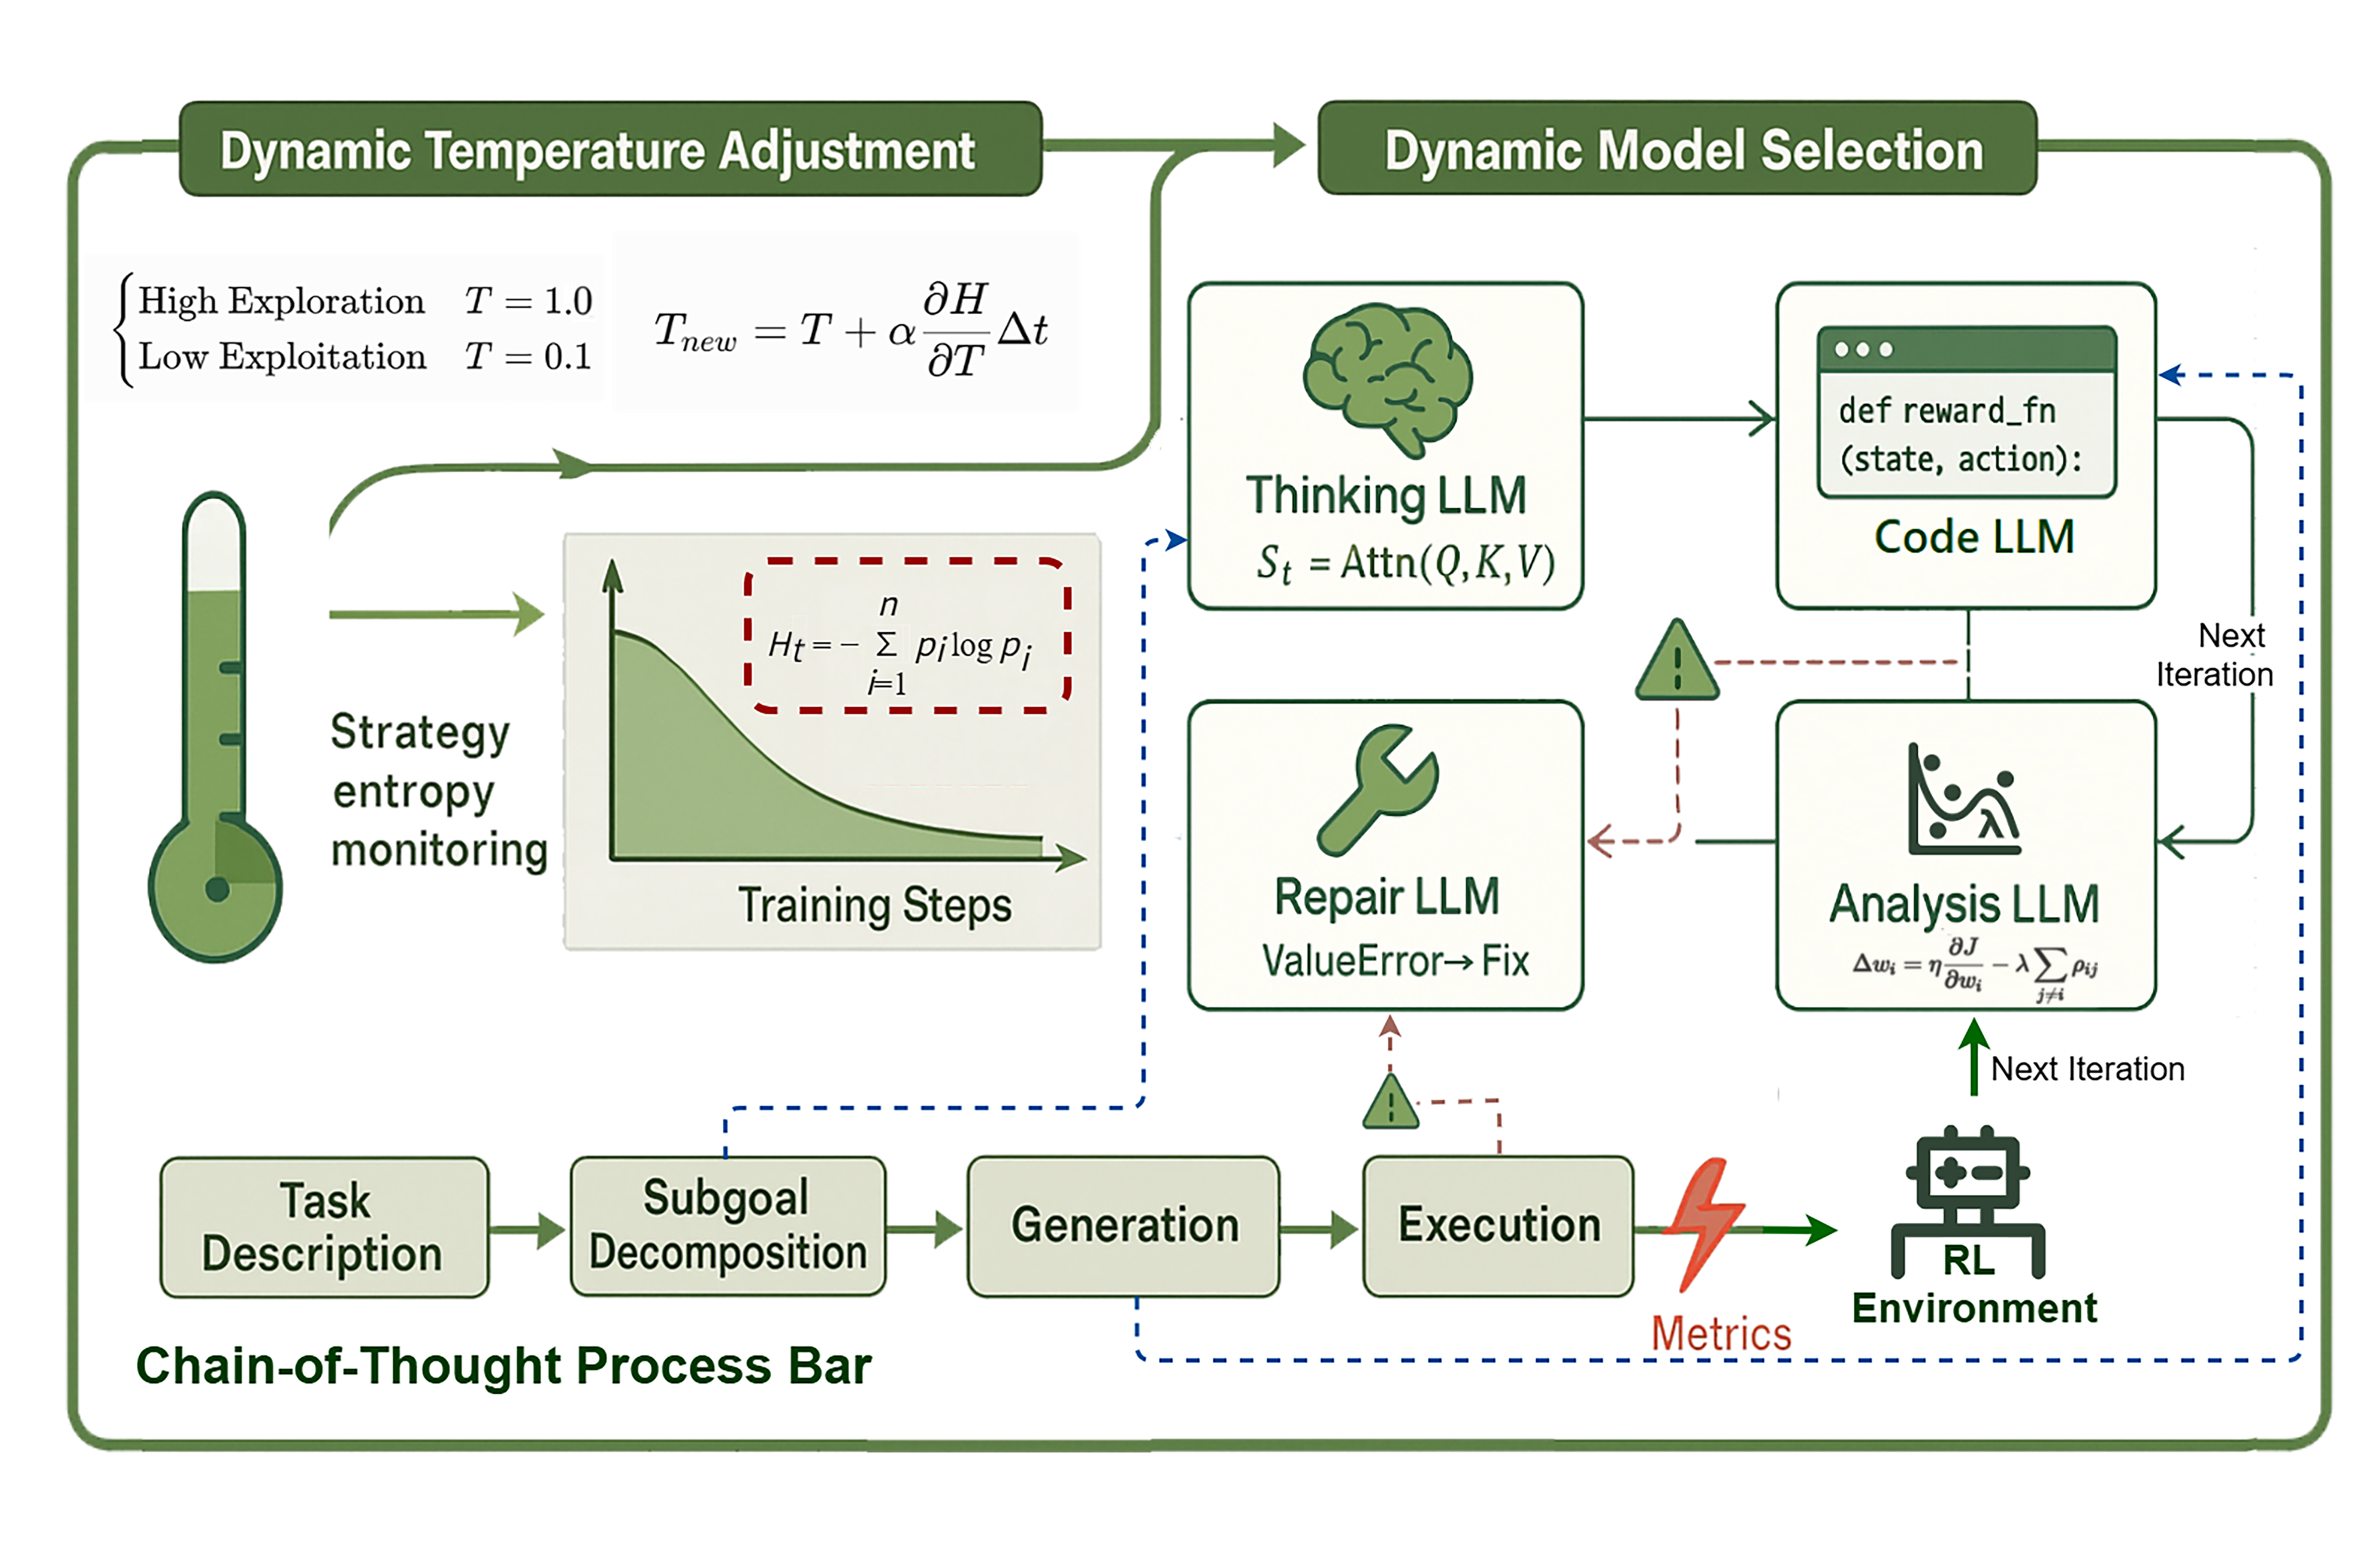
\includegraphics[width=0.95\linewidth]{Figures/dycot-re-control-flow.png}
    \caption{DyCoT-RE control flow integrating temperature modulation and model selection within CoT iterative reasoning.}
    \label{fig:control-flow}
\end{figure*}

\subsubsection{Dynamic Temperature Adjustment}

Temperature adjustment modulates the sampling temperature $T$ 
based on policy entropy $H$, confidence $C$, and performance $R$. 
Entropy reflects generative diversity, confidence measures output stability, 
and performance evaluates reward improvement relative to historical best.

The update rule is formulated as:

\begin{equation}
T_{k+1}
=
\text{clip}
\left(
T_k
+
\alpha \frac{\partial T}{\partial H_k} \Delta t
\right),
\end{equation}

where $\alpha$ is a learning rate,
and the gradient $\frac{\partial T}{\partial H_k}$ reflects entropy-driven adjustment.
An alternative implementation combines smoothing and multiplicative adjustment:

\begin{equation}
T_{k+1}
=
\text{clip}
\left(
\alpha T_k
+
(1-\alpha) T_k f(H_k,C_k,R_k)
\right).
\end{equation}

Here, $f(H,C,R)$ integrates:

\begin{equation}
f(H,C,R)
=
f_R(R)
f_H(H)
f_C(C),
\end{equation}

where $f_R$ ensures performance protection, $f_H$ regulates entropy bounds,
and $f_C$ maintains confidence stability.

\subsubsection{Dynamic Model Selection}

Dynamic model selection adaptively routes sub-tasks to specialized LLMs, 
leveraging their complementary strengths across the reward engineering pipeline.

The four LLM classes include:
$\mathcal{M}_{\text{think}}$ for task understanding and semantic decomposition, 
$\mathcal{M}_{\text{code}}$ for reward function synthesis, 
$\mathcal{M}_{\text{repair}}$ for code correction, 
and $\mathcal{M}_{\text{analysis}}$ for performance evaluation and sub-reward weight updates.

Formally, the decomposition and generation process can be expressed as:

\begin{equation}
g_i = \mathcal{M}_{\text{think}}(d,E),
\end{equation}

\begin{equation}
w_i = \mathcal{M}_{\text{analysis}}(R_i),
\end{equation}

\begin{equation}
r_i(s,a) = \mathcal{M}_{\text{code}}(g_i,w_i),
\end{equation}

where $d$ is the task description and $E$ the environment specification.
Repair LLM intervenes when $\mathcal{M}_{\text{code}}$ outputs execution errors during evaluation.

Model selection at iteration $k$ follows:

\begin{equation}
    M_{k+1} =
    \begin{cases}
    \displaystyle
    \arg\max_{m \in \mathcal{M}_s} \text{Perf}(m), & 1-\epsilon, \\[8pt]
    \text{Random}(\mathcal{M}_s \setminus \{M_k\}), & \epsilon,
    \end{cases}
    \end{equation}
    

where $\mathcal{M}_s$ is the model pool for stage $s$, 
$\text{Perf}(m)$ the performance score, 
and $\epsilon$ the exploration rate ensuring selection diversity.

At each iteration, the next model $M_{k+1}$ is selected by choosing the highest-performing model from the pool $\mathcal{M}_s$ with probability $1-\epsilon$, or randomly selecting another model with probability $\epsilon$. This pool includes the Repair LLM, which is triggered when error correction is needed during reward code evaluation.

\subsubsection{Joint Adaptive Optimization}

Temperature adjustment and model selection form a joint adaptive optimization loop.
Temperature $T$ influences the sampling distribution of reward candidates:

\begin{equation}
r_i(s,a) \sim p(r_i | g_i, T),
\end{equation}

where $g_i = \mathcal{M}_{\text{think}}(d,E)$ denotes the subgoal generated by the Thinking LLM
given task description $d$ and environment $E$.
This sampling process modulates policy entropy and, consequently, cumulative rewards.

Concurrently, model selection determines the semantic decomposition quality,
code correctness, error repair, and performance evaluation,
thereby shaping the expressivity and effectiveness of reward functions.

The combined objective of temperature adjustment and model selection is to maximize:

\begin{equation}
J(\theta; T, M)
=
\mathbb{E}_{\pi_\theta}
\left[
\sum_{t=0}^{T}
\gamma^t
R_{T,M}(s_t,a_t)
\right],
\end{equation}

where $R_{T,M}(s,a)$ is the reward function generated under temperature $T$
and model configuration $M$.

This joint optimization is formalized as:

\begin{equation}
(T^*, M^*)
=
\arg\max_{T,M}
J(\theta; T, M).
\end{equation}

Overall, this interconnected loop iteratively adapts both sampling temperature
and model selection strategies to maximize the expected RL objective
as defined in Eq.~\eqref{eq:rl_objective}, ensuring stable, diverse,
and effective reward engineering throughout the training process.




\section{Experiments}


\subsection{Experimental Setup}


DyCoT-RE is evaluated on four reinforcement learning environments,
which span diverse task difficulties, action spaces, and generalization challenges.

Standard benchmarks include CartPole, BipedalWalker, and Ant,
covering discrete control tasks and high-dimensional continuous locomotion.

To assess generalization beyond pretrained benchmark knowledge,
we introduce SpaceMining, a custom-designed environment
where an agent collects resources under partial observability
and dynamic physics constraints.

SpaceMining is developed as an original contribution in this work,
with full code released and interactive visualizations available on the project website.


\subsubsection{Baselines}

We evaluate DyCoT-RE against two representative baselines to contextualize its performance:

\textbf{(1) Human-designed rewards}  
Standard expert-crafted reward functions using Gymnasium's native implementations for CartPole, BipedalWalker, and Ant, 
with manual heuristics for SpaceMining. This reflects the traditional gold standard in RL.

\textbf{(2) Eureka}  
A LLM-based framework that demonstrated LLMs' potential in automated reward design through code synthesis and verification. 
As a foundational work in this space, it provides a natural reference for assessing our incremental improvements. 
While Eureka focuses on direct code generation without CoT or dynamic optimization, we adapt its pipeline to our Gymnasium-based 
evaluation settings for consistency.

Additionally, to assess the contribution of each DyCoT-RE module, Section~\ref{sec:ablation} conducts ablation studies 
comparing DyCoT-RE against its internal variants:

- Zero-shot reward generation without CoT reasoning

- DyCoT-RE without temperature adjustment

- DyCoT-RE without model selection



\subsubsection{Implementation Details}

All experiments use Proximal Policy Optimization from Stable-Baselines3, with hyperparameters summarized in Table~\ref{tab:env_specs}.

Training uses the Adam optimizer with a learning rate of 0.0003, batch size 64, $\lambda=0.95$, and $\gamma=0.999$.

Reward functions are generated by DyCoT-RE with a local LLM deployed via Ollama. Each chain-of-thought iteration samples eight candidate rewards in parallel with a temperature of 0.6 to balance diversity and coherence.

Final performance is reported as the mean over ten test episodes with different seeds.

\begin{table}[ht]
\centering
\caption{Environment Specifications}
\label{tab:env_specs}
\begin{tabular}{lcccc}
\toprule
Environment & State & Action & Steps & Key Features \\
\midrule
CartPole & 4D & 1D (disc) & 500 & Balance \\
BipedalWalker & 24D & 4D (cont) & 1600 & Locomotion \\ 
Ant & 111D & 8D (cont) & 1600 & Multijoint \\
SpaceMining & 71D & 4D (cont) & 1600 & 3D mining \\
\bottomrule
\end{tabular}
\end{table}



\subsection{Performance Across Environments}

This section evaluates DyCoT-RE relative to baseline methods, focusing on its effectiveness and convergence efficiency.

\begin{figure}[ht]
\centering
\includegraphics[width=0.9\textwidth]{Figures/bar_comparison_5.pdf}
\caption{Final average rewards comparing Human-designed, Eureka, and DyCoT-RE across environments.}
\label{fig:bar_comparison}
\end{figure}

Figure~\ref{fig:bar_comparison} shows that DyCoT-RE achieves comparable or higher final rewards in all tasks. The improvement is most prominent in Ant and SpaceMining, where sparse feedback and complex task structures limit the effectiveness of handcrafted rewards.

\begin{figure}[t]
\centering
\includegraphics[width=0.9\textwidth]{Figures/reward_episode_curve_3.pdf}
\caption{Learning curves for DyCoT-RE (blue), Human-designed (dark green), and Eureka (light green).}
\label{fig:learning_curves}
\end{figure}

Figure~\ref{fig:learning_curves} illustrates training dynamics across environments. In CartPole, all methods reach high rewards quickly, but DyCoT-RE converges with fewer iterations. BipedalWalker learning is smoother under DyCoT-RE, suggesting benefits from structured reward decomposition that disentangles balance and propulsion. Ant shows a gradual reward increase under DyCoT-RE while baselines plateau earlier, implying improved credit assignment in high-dimensional control. In SpaceMining, DyCoT-RE maintains a steady reward increase while other methods show little progress, reflecting its adaptability to novel task domains without predefined heuristics.

\begin{table}[htbp]
\centering
\caption{Final rewards, average convergence episodes (k), and success rates over 50 runs comparing DyCoT-RE and Eureka. Human-designed results included without convergence data.}
\label{tab:perf_summary_simple}
\begin{tabular}{lccc}
\hline
Environment & Method  & Conv . & Success (\%) \\
\hline
CartPole 
& DyCoT-RE  & 2.7 & 100 \\
& Eureka    & 3.8 & 95 \\

BipedalWalker 
& DyCoT-RE & 5.6 & 98 \\
& Eureka   & 6.9 & 92 \\

Ant 
& DyCoT-RE & 11.5 & 85 \\
& Eureka   & 14.2 & 72 \\

SpaceMining 
& DyCoT-RE & 7.1 & 88 \\
& Eureka   & 9.6 & 65 \\
\hline
\end{tabular}
\end{table}
    

Table~\ref{tab:perf_summary_simple} compares DyCoT-RE with Eureka and Human-designed baselines. Across all four environments, DyCoT-RE achieves the highest final rewards and fastest convergence, with success rates exceeding 85% in each task. Notably, late-stage gain values reveal that DyCoT-RE maintains continued performance improvements during the final training stages, whereas Human-designed rewards tend to saturate early.

These results indicate that DyCoT-RE’s integration of Chain-of-Thought reasoning with dynamic optimization leads to faster learning and higher rewards, particularly in tasks with sparse signals or novel objectives. Its ability to decompose complex tasks into semantically meaningful sub-rewards facilitates efficient policy learning without extensive manual reward shaping.

\subsection{Ablation Study}
\label{sec:ablation}

This section conducts an ablation study to examine the individual contribution of each component in DyCoT-RE, including CoT reasoning, temperature adjustment, and model selection, as well as their combined synergistic effects.

\subsubsection{Impact of CoT Reasoning}


We evaluate the impact of incorporating Chain-of-Thought (CoT) reasoning into reward engineering by comparing DyCoT-RE's CoT-enabled variant against a zero-shot baseline lacking structured intermediate reasoning.



Figure~\ref{fig:cot_ablation} summarizes reward distributions for both methods across the four benchmark environments. A consistent pattern emerges: CoT-enabled rewards exhibit higher means, lower variance, and reduced outlier incidence compared to zero-shot. In CartPole and SpaceMining, CoT-enabled results are tightly clustered near the environment's upper performance bounds, whereas zero-shot results are widely dispersed, with a substantial proportion of runs yielding suboptimal or even near-zero rewards. This reflects CoT's ability to systematically decompose task objectives into interpretable sub-rewards, enhancing sample efficiency and stabilizing policy learning.



\begin{figure}[ht]
    \centering
    \includegraphics[width=0.9\textwidth]{Figures/cot_ablation_2.pdf}
    \caption{Final reward distributions for CoT-enabled vs zero-shot reward generation across environments.}
    \label{fig:cot_ablation}
    \end{figure}

In BipedalWalker, an illustrative deviation is observed. While CoT-enabled runs achieve rewards concentrated between 250–310 with minimal negative outcomes, zero-shot results present a bimodal distribution: one cluster achieves moderate positive rewards ($\sim$150–250), while another cluster yields severely negative rewards (e.g. -124, -97, -73). This bimodality indicates that without structured reasoning, reward generation often fails to encode essential balance or locomotion constraints, resulting in policies that collapse during gait training.


Taken together, these results illustrate that CoT reasoning reliably improves reward interpretability and training stability, especially in settings with sparse or ambiguous feedback.


    


\subsubsection{Impact of Temperature Adjustment}


Due to computational constraints and consistent observed trends across environments, 
temperature adjustment and model selection ablation were conducted on BipedalWalker as a representative continuous control task, 
while CoT reasoning was evaluated on all four environments to confirm its general effectiveness.

This section investigates the effect of temperature settings by sweeping $T \in [0.0, 1.0]$ on the BipedalWalker environment. 

Table~\ref{tab:temp_sweep} summarizes the results, including average fitness, maximum/minimum fitness, standard deviation, and reward efficiency ratio (average fitness divided by standard deviation).

\begin{table}[ht]
\centering
\caption{BipedalWalker performance under different temperature settings. Top-1 temperature is highlighted in green, DyCoT-RE result in blue.}
\label{tab:temp_sweep}
\begin{tabular}{c|c|c|c|c}
\hline
Temp & Avg Fit$\uparrow$ & Max/Min Fit $\uparrow$& Std$\downarrow$  & Eff. Ratio$\uparrow$ \\
\hline
0.0 & 81.93 & 301.15/-53.01 & 148.67 & 0.55 \\
0.1 & 149.56 & 310.94/-33.73 & 155.22 & 0.96 \\
0.2 & 242.74 & 313.60/-20.27 & 125.47 & 1.93 \\
0.3 & 210.07 & 311.17/-46.69 & 140.49 & 1.50 \\
\rowcolor{green!15}
0.4 & 244.19 & 311.94/-17.13 & 107.02 & 2.28 \\
0.5 & 215.84 & 310.69/-14.25 & 131.01 & 1.65 \\
\rowcolor{green!25}
0.6 & 248.11 & 312.48/-21.18 & 120.45 & 2.06 \\
0.7 & 225.88 & 312.42/-12.08 & 131.43 & 1.72 \\
0.8 & 74.33 & 310.42/-46.72 & 143.91 & 0.52 \\
0.9 & 145.02 & 310.02/-31.58 & 148.51 & 0.98 \\
1.0 & 192.38 & 310.40/-39.05 & 138.37 & 1.39 \\
\rowcolor{blue!15}
DyCoT-RE & \textbf{292.8} & 315.6/87.2 & 55.2 & 5.30 \\
\hline
\end{tabular}
\end{table}

Static sweeps show that mid-range temperatures ($T=0.4$–$0.6$) yield higher fitness and lower variance than extremes. 
DyCoT-RE’s dynamic temperature regulation consistently outperforms these static settings, 
adapting temperature during training to maintain an effective exploration-exploitation trade-off. 


\subsubsection{Impact of Model Selection}

Finally, we evaluate the impact of DyCoT-RE's dynamic model selection by comparing it against individual static LLM baselines on the BipedalWalker environment. Table~\ref{tab:model_selection} summarizes average fitness, max/min fitness, standard deviation, and reward efficiency ratio (average fitness divided by standard deviation). Only models with sufficient sample sizes ($N>10$) are included.

DyCoT-RE achieves the highest average fitness (\cellcolor{blue!15}307.28) with exceptionally low standard deviation (\cellcolor{blue!15}6.00) and the best efficiency ratio (\cellcolor{blue!15}51.21), demonstrating its capability to consistently generate high-quality rewards across diverse sub-tasks. 

In contrast, while \texttt{codegemma} achieves competitive performance (Avg Fit: 260.8), its higher standard deviation (115.2) results in a substantially lower efficiency ratio (2.26), indicating reduced stability and generalizability compared to DyCoT-RE.

\begin{table}[ht]
\centering
\caption{Performance comparison of different LLM backends (N=20) in BipedalWalker. $\uparrow$: higher is better; $\downarrow$: lower is better. Green: per-column best baseline. Blue: DyCoT-RE (dynamic selection).}
\label{tab:model_selection}
\begin{tabular}{l|c|c|c|c}
\hline
Model (size) & Avg Fit $\uparrow$ & Max Fit $\uparrow$ & Std $\downarrow$ & Eff. Ratio $\uparrow$ \\
\hline
codegemma (7b) & 260.8 & 301.8 & \cellcolor{green!25}34.2 & 3.46\cellcolor{green!25} \\
codeqwen (7b) & 32.6 & 307.6 & -76.0 & 0.33 \\
deepseek-coder (6.7b) & -4.5 & 295.3 & -98.2 & -0.05 \\
deepseek-r1 (8b) & 44.6 & \cellcolor{green!25}321.2 & -99.6 & 0.37 \\
gemma3 (4b) & \cellcolor{green!25}278.0 & 314.8 & -34.2 & 3.39 \\
llama3.1 (8b) & 162.2 & 318.4 & -80.4 & 1.08 \\
qwen2.5 (7b) & 177.0 & 319.5 & -97.2 & 1.17 \\
qwen2.5-coder (7b) & 125.6 & 313.7 & -70.8 & 0.77 \\
\rowcolor{blue!15}
DyCoT-RE & \textbf{297.28} & \textbf{316.57} & \textbf{89.47} & \textbf{6.46} \\
\hline
\end{tabular}
\end{table}

While individual models occasionally excel on narrow tasks, DyCoT-RE’s dynamic model routing provides the most generalizable performance, 
effectively balancing reward quality, stability, and adaptability in complex continuous control environments.

In summary, the ablation study demonstrates that each module—CoT reasoning, temperature adjustment, and model selection—contributes significantly to DyCoT-RE’s superior performance, and their combination leads to synergistic gains.

\subsection{SpaceMining Performance and Reward Decomposition Analysis}

The SpaceMining environment was specifically designed to evaluate DyCoT-RE in scenarios lacking prior task-specific knowledge. Unlike standard benchmarks such as CartPole or Ant, which share dynamics and reward structures commonly encountered in pretraining corpora, SpaceMining introduces a novel multi-objective resource collection task with sparse and delayed rewards, dynamic obstacles, and energy constraints. This setup aims to assess whether DyCoT-RE can generate effective reward functions purely based on task descriptions without relying on pretrained knowledge templates.

\begin{figure}[ht]
    \centering
    \includegraphics[width=0.9\linewidth]{Figures/dynamics_overview.pdf}
    \caption{Training progress in SpaceMining: multi-dimensional metrics over 3M timesteps. Reward (blue), energy (dark green), and inventory (light green) reflect task-specific learning dynamics.}
    \label{fig:space_mining_multivariate}
\end{figure}

Figure~\ref{fig:space_mining_multivariate} demonstrates DyCoT-RE’s performance in the custom-designed SpaceMining environment. 
The reward curve exhibits an initial exploration plateau, a phase of stable increase corresponding to effective policy acquisition, 
and a final convergence to near-maximal performance. 
Energy shows a smooth decreasing trend due to continuous task execution, while inventory displays cyclical fluctuations representing 
mining and delivery loops.

\subsubsection{Reward Decomposition Design and Quantitative Contributions}

Table~\ref{tab:space_mining_rewards} summarizes the reward decomposition designed by DyCoT-RE for SpaceMining. 
Each sub-reward component is listed with its computation formula, assigned weight coefficient, and empirical contribution ratio 
calculated over the final training stage.

\begin{table}[ht]
\centering
\caption{Reward decomposition components in SpaceMining with formula, coefficient, and empirical contribution.}
\label{tab:space_mining_rewards}
\begin{tabular}{llll}
\hline
Sub-reward & Computation Formula & Weight & Contribution \\
\hline
Mining & $\log(1+\text{mined\_amount})$ & 0.4 & 38.2\% \\
Delivery & $\text{delivered\_amount} \cdot e^{-d/D}$ & 0.3 & 35.1\% \\
Exploration & $\mathbb{I}(\text{new\_asteroid}) \cdot 0.1$ & 0.2 & 15.7\% \\
Energy Conservation & $\text{energy\_remaining}/E_{max}$ & 0.2 & 22.0\% \\
Collision Penalty & $- \lVert \text{collision} \rVert^2$ & -0.1 & -11.0\% \\
\hline
\end{tabular}
\end{table}

The decomposition captures task semantics effectively. Mining and delivery sub-rewards dominate, aligning with primary objectives of resource extraction and transport. Exploration provides auxiliary guidance, while energy conservation ensures operational efficiency. The negative collision penalty maintains safety compliance with minimal policy interference.

DyCoT-RE’s structured decomposition thus enables interpretable and modular reward design, translating high-level task requirements into quantitative objectives that facilitate effective agent training in novel, out-of-distribution environments such as SpaceMining.


\section{Discussion}

This work presents DyCoT-RE, a reward engineering framework combining Chain-of-Thought reasoning, dynamic temperature regulation, and adaptive model selection. Experiments across four RL tasks show DyCoT-RE consistently outperforms heuristic rewards and automated baselines like Eureka, especially in complex, sparse-reward environments such as Ant and SpaceMining. For simpler tasks like CartPole, gains are smaller due to already dense rewards.
Ablation results highlight that CoT reasoning improves reward interpretability and stability, dynamic temperature adjustment enhances sample efficiency over static settings, and adaptive model selection reduces variance by leveraging multiple LLMs effectively.

Despite these strengths, DyCoT-RE has limitations. Its reliance on LLM inference introduces computational overhead, and performance may degrade if backend models lack domain-relevant priors. Furthermore, while Chain-of-Thought reasoning improves reward decomposition quality, its efficacy remains sensitive to prompt design and reasoning chain depth, especially in novel environments without structured knowledge templates.

Future work could explore integrating DyCoT-RE with offline reinforcement learning to reduce online sampling costs, extending model selection mechanisms to multimodal backends for vision-language task settings, and applying human-in-the-loop evaluation to refine interpretability metrics beyond decomposition-based heuristics. Additionally, broader testing on diverse real-world tasks, such as industrial robotics and multi-agent coordination, will help assess the framework's scalability and general applicability.

In summary, DyCoT-RE advances the automated design of reward functions by combining cognitive reasoning paradigms with dynamic optimization mechanisms, showing promise as a practical tool for scalable and interpretable reinforcement learning across task domains of varying complexity.

\section{Conclusion}

This paper presented DyCoT-RE, a reward engineering framework that integrates Chain-of-Thought reasoning, dynamic temperature regulation, and adaptive model selection to automate reward function design in reinforcement learning. Evaluations across a variety of tasks—from simple discrete control to complex continuous locomotion and resource collection—show that DyCoT-RE consistently outperforms human-designed heuristics and prior automated methods.

The experiments demonstrate that Chain-of-Thought reasoning improves the quality of reward decomposition, dynamic temperature adjustment enhances sample efficiency, and adaptive model selection contributes to more stable and generalizable performance. The combined effect of these components enables DyCoT-RE to better handle sparse, ambiguous, or novel task environments while maintaining stable training.

The approach requires additional computational resources and depends on the availability of capable language models. Future research will explore integration with offline reinforcement learning, expansion to multi-agent and vision-language domains, and incorporation of human feedback to better align reward design with user intent.

Overall, DyCoT-RE advances automated reward design by combining cognitive reasoning with dynamic optimization techniques, offering a pathway toward scalable and robust reinforcement learning across diverse tasks.

\bibliographystyle{elsarticle-num} % 或其他你需要的样式
\bibliography{adaptive_cot_reward_rl} % 不需要加.bib扩展名

\end{document}
